% Standalone RND pipeline figure for Train run 5. Compile: latexmk -pdf rnd_pipeline.tex
% Original RND data flow (solid spine), with CleanRL departures as dashed callouts. The predictor
% gradient path is dashed and terminates ONLY at the predictor; RMS statistic updates are dotted.
\documentclass[tikz,border=6pt]{standalone}
\usepackage{amsmath}
\usepackage{amssymb}
\usetikzlibrary{arrows.meta,positioning,fit,backgrounds,calc}
\begin{document}
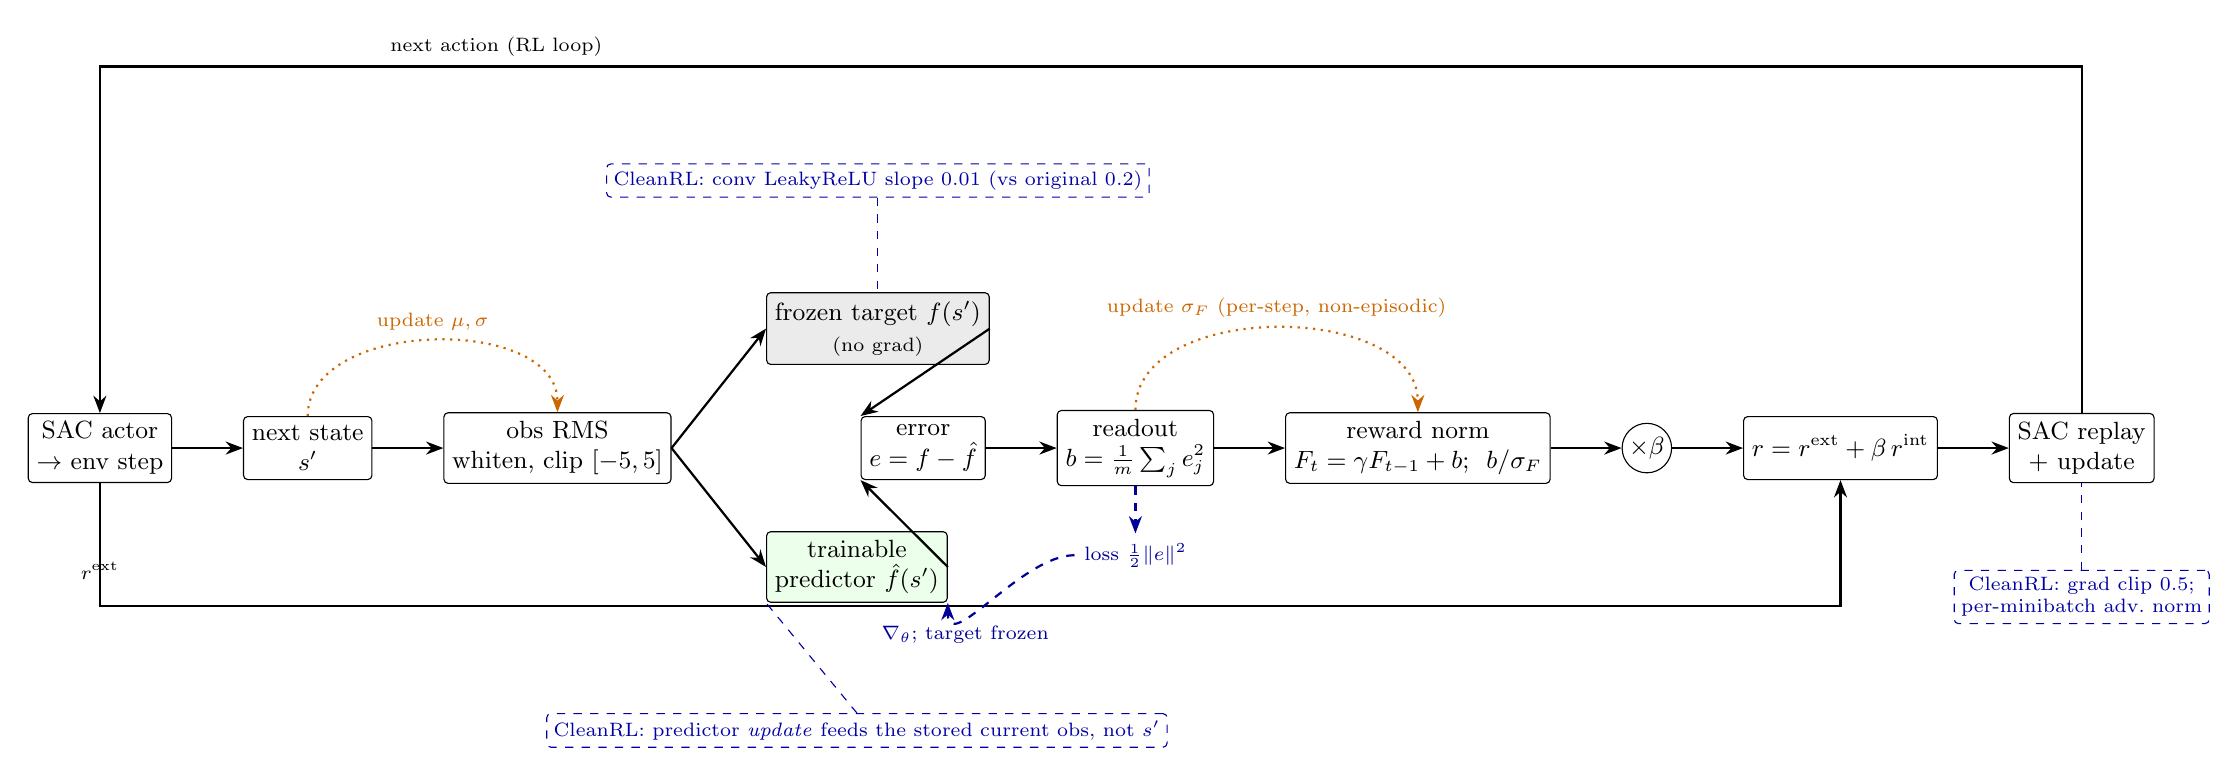
\begin{tikzpicture}[
  font=\small,
  >={Stealth[length=2.2mm]},
  box/.style={draw,rounded corners=1.5pt,align=center,inner sep=3pt,minimum height=8mm,fill=white},
  frozen/.style={box,fill=black!8},
  pred/.style={box,fill=green!8},
  op/.style={draw,circle,inner sep=1pt,minimum size=6mm,fill=white},
  flow/.style={->,thick},
  grad/.style={->,dashed,thick,blue!60!black},
  stat/.style={->,dotted,thick,orange!80!black},
  callout/.style={draw,dashed,rounded corners=1.5pt,align=center,font=\scriptsize,inner sep=2.5pt},
  cleanrl/.style={callout,blue!65!black},
  node distance=7mm and 9mm,
]
% ---- main spine (left to right) ----
\node[box] (env) {SAC actor\\$\to$ env step};
\node[box,right=of env] (s) {next state\\$s'$};
\node[box,right=of s] (norm) {obs RMS\\whiten, clip $[-5,5]$};
% target above, predictor below the spine, both fed by norm and feeding the error
\node[frozen,above right=6mm and 12mm of norm] (tgt) {frozen target $f(s')$\\{\scriptsize(no grad)}};
\node[pred,below right=6mm and 12mm of norm] (prd) {trainable\\predictor $\hat f(s')$};
\node[box,right=24mm of norm] (err) {error\\$e=f-\hat f$};
\node[box,right=of err] (read) {readout\\$b=\tfrac1m\sum_j e_j^2$};
\node[box,right=of read] (rnorm) {reward norm\\$F_t=\gamma F_{t-1}+b$;\ \ $b/\sigma_F$};
\node[op,right=of rnorm] (beta) {$\times\beta$};
\node[box,right=of beta] (sum) {$r=r^{\mathrm{ext}}+\beta\,r^{\mathrm{int}}$};
\node[box,right=of sum] (rl) {SAC replay\\$+$ update};
% ---- forward edges ----
\draw[flow] (env) -- (s);
\draw[flow] (s) -- (norm);
\draw[flow] (norm.east) -- (tgt.west);
\draw[flow] (norm.east) -- (prd.west);
\draw[flow] (tgt.east) -- (err.north west);
\draw[flow] (prd.east) -- (err.south west);
\draw[flow] (err) -- (read);
\draw[flow] (read) -- (rnorm);
\draw[flow] (rnorm) -- (beta);
\draw[flow] (beta) -- (sum);
\draw[flow] (sum) -- (rl);
% ---- extrinsic reward bypass (env -> sum): flat orthogonal route below the predictor box ----
\draw[flow] (env.south) |- ($(sum.south)+(0,-1.6)$) node[pos=0.28,below,font=\scriptsize]{$r^{\mathrm{ext}}$} -| (sum.south);
% ---- RL loop back-edge: flat orthogonal route ABOVE all callouts; label at the far right ----
\draw[flow] (rl.north) |- ($(env.north)+(0,4.4)$) node[pos=0.9,above,font=\scriptsize]{next action (RL loop)} -| (env.north);
% ---- predictor gradient path (dashed, terminates at predictor only) ----
\node[below=6mm of read,font=\scriptsize,blue!60!black] (loss) {loss $\tfrac12\lVert e\rVert^2$};
\draw[grad] (read.south) -- (loss.north);
\draw[grad] (loss.west) to[out=180,in=-90] node[below,pos=0.7,font=\scriptsize]{$\nabla_{\theta}$; target frozen} (prd.south east);
% ---- RMS statistic-update paths (dotted) ----
\draw[stat] (s.north) to[out=90,in=90] node[above,pos=0.5,font=\scriptsize]{update $\mu,\sigma$} (norm.north);
\draw[stat] (read.north) to[out=90,in=90] node[above,pos=0.5,font=\scriptsize]{update $\sigma_F$ (per-step, non-episodic)} (rnorm.north);
% ---- CleanRL departure callouts (placed in whitespace, short leaders) ----
\node[cleanrl,above=12mm of tgt] (c1) {CleanRL: conv LeakyReLU slope $0.01$ (vs original $0.2$)};
\draw[dashed,blue!65!black] (c1.south) -- (tgt.north);
\node[cleanrl,below=14mm of prd] (c2) {CleanRL: predictor \emph{update} feeds the stored current obs, not $s'$};
\draw[dashed,blue!65!black] (c2.north) -- (prd.south west);
\node[cleanrl,below=11mm of rl] (c3) {CleanRL: grad clip $0.5$;\\per-minibatch adv.\ norm};
\draw[dashed,blue!65!black] (c3.north) -- (rl.south);
\end{tikzpicture}
\end{document}
